\chapter{DESENVOLVIMENTO DA APLICAÇÃO}
%https://rafaell-lycan.com/2015/construindo-restful-api-laravel-parte-1/

O presente trabalho apresenta uma API REST, a qual possibilita a coleta das coordenadas geográficas dos pedidos gerados nos estabelecimentos. Além disso, apresenta o desenvolvimento de uma aplicação para gerenciar, por meio de um painel de controle, a logística das entregas de comida, próteses, entre outras mercadorias. Tal aplicação tem por objetivo fornecer ao motoboy um módulo de entregas, possibilitando a ele observar no mapa a rota e os pontos de parada que devem ser percorridos. Todo o processo de comunicação da aplicação ocorre totalmente em tempo real, o que possibilita agilidade e segurança quanto ao destino final.

\section{Softwares utilizados}

Esta Seção apresenta os softwares utilizados na etapa de codificação da aplicação. Para diminuir o custo de desenvolvimento, optou-se pela utilização de tecnologias gratuitas. 
%Outro importante ponto na escolha das ferramentas é a questão de documentação disponível na comunidade web.

\begin{itemize}
    \item PhpStorm: IDE completa de desenvolvimento para projetos codificados com a linguagem de programação PHP;
    \item Composer: gerenciador de pacotes em nível de aplicativo, que fornece um formato padrão para gerenciar dependências de software PHP e bibliotecas necessárias;
    \item Cmder: console para execução de linhas de comandos para o sistema operacional Windows. Com essa ferramenta é possível executar comandos Unix diretamente no Windows;
    \item Laravel: \textit{framework} de programação baseada na linguagem PHP;
    \item Artisan CLI: interface de linha de comando incluída no Laravel, fornecendo vários comandos úteis durante a criação da aplicação, por exemplo: configuração de ambiente, verificar rotas, interagir com a aplicação e criar diversos tipos de arquivos (\textit{Migrations}, \textit{Controllers} e \textit{Models});
    \item Blade: ferramenta para criação de interfaces gráficas, utilizado pelo Laravel como uma ferramenta de \textit{template}, trazendo uma quantidade grande de funcionalidades que ajudam na criação de interfaces interativas;
    \item Eloquent ORM: ferramenta com funcionalidades que facilitam a inserção, atualização, busca e exclusão de registros diretamente no banco de dados;
    \item XAMPP: servidor independente de plataforma, que inclui: Apache, MySQL, phpMyAdmin, FileZilla FTP Server, OpenSSL, PHP e Perl;
    \item Jaspersoft Studio: ferramenta para projetar e executar modelos de relatório com expressões, gráficos, mapas, tabelas e \textit{QR Codes}, criando documentos de qualquer complexidade a partir de informações presentes no banco de dados;
    \item GitHub: plataforma de hospedagem de código-fonte para controle de versão;
    \item Sourcetree: representação visual de repositórios da nuvem.
\end{itemize}

\newpage
Para o desenvolvimento deste trabalho, foi escolhido trabalhar com Laravel 5.8.11, um \textit{framework} com um servidor interno já incluso e invocado através do comando \textit{php artisan serve}, em conjunto com o XAMPP, o que facilita e agiliza o desenvolvimento. Como o conteúdo estará armazenado na rede local, o acesso aos arquivos é realizado instantaneamente, ficando disponível no endereço \textit{http://127.0.0.1}.

A execução do comando \textit{composer create-project --prefer-dist laravel/laravel delivery-routes} no Cmder gera, de forma padronizada, toda a estrutura de um projeto Laravel, apresentada na \autoref{fig:base-projeto}. O uso do Cmder torna o desenvolvimento, via terminal, do sistema operacional Windows mais amigável. Uma vez que esta ferramenta possibilita a execução de comandos Unix em ambiente Microsoft.

\begin{figure}[H]
    \centering
    \caption{Estrutura Laravel}
    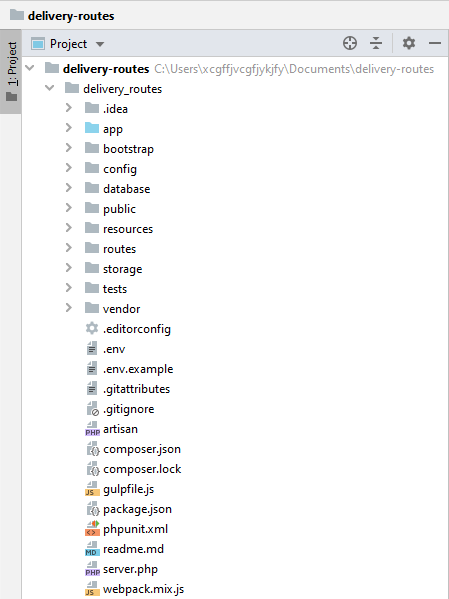
\includegraphics[width=0.48\textwidth]{./dados/figuras/fig6}
    \fonte{Autor}
    \label{fig:base-projeto}
\end{figure}

A montagem do ambiente de desenvolvimento para deixa-lo funcional no \textit{framework} Laravel necessitou de algumas configurações, tais como: primeiramente foi preciso instalar e configurar todas as dependências do PHP para que se pudesse ter acesso a linguagem de programação através do gerenciados de dependências Composer.

Foi optado, por questões de controle de versionamento do projeto, hospedar o código-fonte do projeto em nuvem, através da plataforma GitHub. A sincronia entre os arquivos locais e o GitHub foi possível com o auxílio do sistema de controle de versões chamado Git, representado visualmente pelo Sourcetree, que deixa o trabalho braçal por linha de comando (\textit{gitbash}) de lado, sendo também necessário sua instalação e configuração na máquina de desenvolvimento. 

O banco de dados escolhido para armazenar os registros foi o MySQL, cuja instalação e configuração ocorreu automaticamente pelo XAMPP. Por último, para ter acesso a manipulação do código, um editor de texto era necessário, optando-se pelo PHPStorm. Esta, uma IDE paga, mas utilizando o e-mail acadêmico da URI, obtive a licença estudantil, terminando assim a fase configuração de ambiente de desenvolvimento e garantindo aptidão para começar os trabalhos.

O próximo passo foi a modelagem dos dados, onde verificou-se que seria necessário a criação das seguintes tabelas com o recurso \textit{Migration}: \textit{users}, \textit{motoboys}, \textit{deliveries}, \textit{payments} e \textit{orders}. Uma sexta tabela chamada de \textit{deliveries\_orders} precisou ser criada para vincular mais de um pedido à cada entrega, onde uma \textit{trigger}, disparada via \textit{after update}, ficou responsável pela atualização do status de cada pedido vinculado à entrega, esta chamada de \textit{tr\_Status\_Orders}, apresentada no \autoref{alg:trigger}. Na próxima Seção serão abordados os possíveis status de um pedido.

\begin{lstlisting}[caption={Delivery Routes - Trigger tr\_Status\_Orders}, label=alg:trigger, style=SQL]
CREATE TRIGGER tr_Status_Orders AFTER UPDATE ON `deliveries`
FOR EACH ROW BEGIN
    UPDATE `orders` o SET `status` = NEW.status WHERE `id` IN
        (SELECT `order_id` FROM `deliveries_orders`
        WHERE `delivery_id` = NEW.id); 
END
\end{lstlisting}

O recurso do Laravel chamado Migration, tem por objetivo gerenciar as mudanças estruturais do banco de dados da aplicação. Para cada tabela, coluna ou índice criados no banco de dados, é possível usar a \textit{migration} para fazer essa operação automática, visando organizar e definir uma sequência de criação das tabelas. Para aplicações com poucas tabelas a utilização de \textit{migrations} para gerenciar a estrutura das tabelas é extremamente útil e válida.

O \autoref{alg:migration} demonstra a criação de uma \textit{migration}, por meio do comando \textit{php artisan make:model Delivery -m}. O parâmetro “-m” indica que além do \textit{model}, uma \textit{migration} deve ser criada.
Para atualizar o banco de dados executando todas as \textit{migrations}, é necessário executar o comando \textit{php artisan migrate}. 

\begin{lstlisting}[caption={Delivery Routes - Exemplo de migration}, style=htmlcssjs, label=alg:migration]
 Schema::create('deliveries', function (Blueprint $table) {
    $table->increments('id');
    $table->integer('motoboy_id')->unsigned();
    $table->foreign('motoboy_id')->references('id')->on('motoboys');
    $table->string('status',30);
    $table->timestamps();
});
\end{lstlisting}

%%%Aproveita e comenta sobre seeds, para poder popular tabelas em um ambiente de teste. Cria um seed para uma tabela de tua base e mostra a importancia desta possibilidade para efetuar o desenvolvimento.

\newpage
\section{Módulo de gerenciamento}
 Inicialmente, o objetivo era construir uma aplicação completa para gestão de vendas, focando na geração do pedido e entrega, sendo essa para qualquer ramo de atividade. Porém descobriu-se a possibilidade de um nicho de mercado ainda não explorado e sem concorrentes, em que não é preciso disputar clientes com grandes empresas renomadas e maduras no assunto.
 
 A aplicação desenvolvida foca no gerenciamento das rotas de entregas dos pedidos gerados via e-PDV já operantes, necessitando apenas da disponibilização de uma API no formato de arquivo JSON (\autoref{fig:drHttpAPI}), essa compondo-se de dados essenciais para realização da integração automática abordada na próxima Seção.
 
  \begin{figure}[H]
    \centering
    \caption{Delivery Routes - Requisição HTTP}
    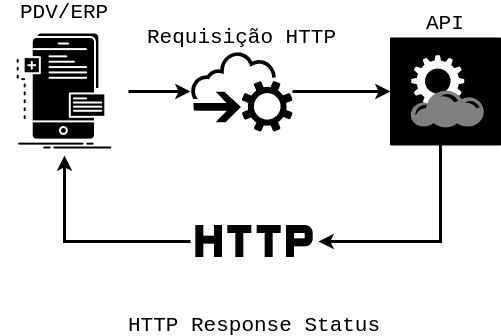
\includegraphics[width=0.6\textwidth]{./dados/figuras/fig16}
    \fonte{\citeonline{iFood}}
    \label{fig:drHttpAPI}
\end{figure}
 
 Primeiramente é preciso entender os possíveis status e o fluxo de um pedido integrado na Delivery Routes, ambos representados na \autoref{tab:drStatusPedido} e na \autoref{fig:drStatusPedido}.
 
 \begin{table}[H]
    \centering
    \caption{Delivery Routes - Status do pedido
    \label{tab:drStatusPedido}}
\begin{tabular}{|l|l|}
\hline
\textbf{Status} & \textbf{Descrição} \\ \hline
PLACED & Indica um pedido foi colocado no sistema. \\ \hline
CONFIRMED & Indica um pedido confirmado. \\ \hline
INTEGRATED & Indica um pedido que foi integrado no sistema. \\ \hline
CANCELLED & Indica um pedido que foi cancelado. \\ \hline
DISPATCHED & Indica um pedido que foi despachado ao cliente. \\ \hline
DELIVERED & Indica um pedido que foi entregue. \\ \hline
CONCLUDED & Indica um pedido que foi concluído. \\ \hline
\end{tabular}
    \fonte{\citeonline{iFood}}
\end{table}
 
 \begin{figure}[H]
    \centering
    \caption{Delivery Routes - Fluxo do status do pedido}
    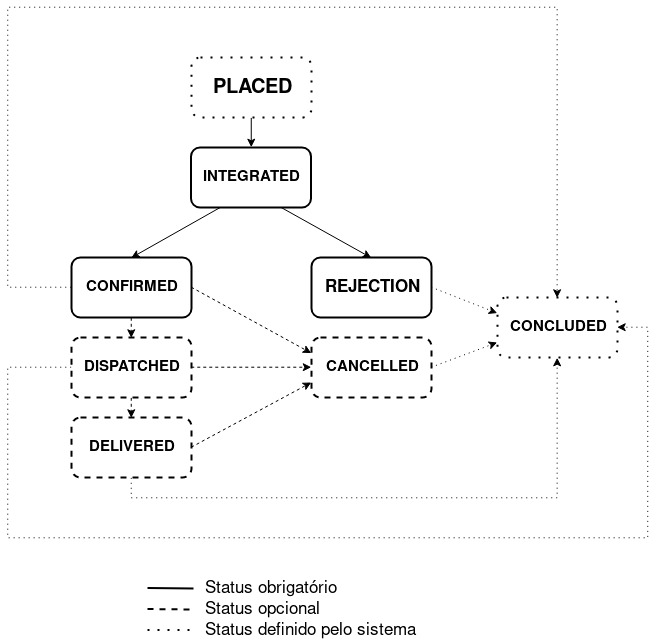
\includegraphics[width=0.6\textwidth]{./dados/figuras/fig15}
    \fonte{\citeonline{iFood}}
    \label{fig:drStatusPedido}
\end{figure}

%%%Se o valor da coluna token_access é diferente ao hash da sessão siginfica que o usuário fez um novo login e gerou um novo hash. Neste caso podemos deslogar o usuário, caso os valores não se coinsidam.

Na \autoref{fig:drLogin} é possível visualizar o acesso ao módulo de gerenciamento, com autenticação apenas para administradores, realizada via e-mail e senha, cujo cadastro é efetuado por meio do link \textit{Register a new membership}. Habilitando a opção \textit{Remember Me}, o controle de única sessão por usuário é ativado, por intermédio de um \textit{hash} gerado no momento do login. É disponibilizado também o link \textit{I forgot my password} para realizar a recuperação da senha, mediante a confirmação de um e-mail existente na base de dados.

\begin{figure}[H]
    \centering
    \caption{Delivery Routes - Login}
    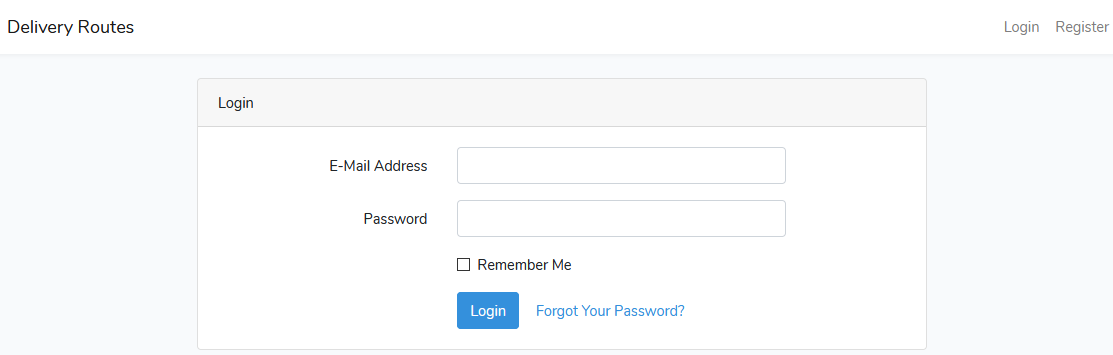
\includegraphics[width=0.4\textwidth]{./dados/figuras/fig7}
    \fonte{Autor}
    \label{fig:drLogin}
\end{figure}

%https://laravel.com/docs/5.7/hashing
O Laravel, juntamente com o Eloquent, disponibiliza a implementação de autenticação de maneira muito simples, por meio do comando \textit{php artisan make:auth}, onde, com poucas instruções e linhas de código, é possível montar a estrutura de cadastro de usuário, recuperação de senha e memória de sessão de maneira extremamente segura, devido ao algoritmo \textit{Bcrypt}
\footnote{Método de criptografia do tipo \textit{hash} adaptativo para senhas que apresenta uma segurança maior em relação à maioria dos outros métodos criptográficos por meio da implementação da variável “custo”, que é proporcional à quantidade de processamento necessária para criptografar a senha \cite{bcrypt}.}
, utilizado para realizar a criptografia da senha.

Ao realizar login, o administrador é apresentado à \textit{dashboard} do sistema, uma interface gráfica que fornece visualização fácil e rápida dos principais indicadores de desempenho, atualizados em tempo real, obtendo assim valores e médias relevantes sobre o processo de negócios. 

Destaca-se na \autoref{fig:drDashboard}, além de indicadores de: Pedidos Em Aberto, Pedidos Em Rota, Motoboys Disponíveis e Pedidos Concluídos, uma barra de menus contendo: Cadastros (Motoboys e Pagamentos) e Movimentos (Entregas e Pedidos Em Aberto).

\begin{figure}[H]
    \centering
    \caption{Delivery Routes - Dashboard}
    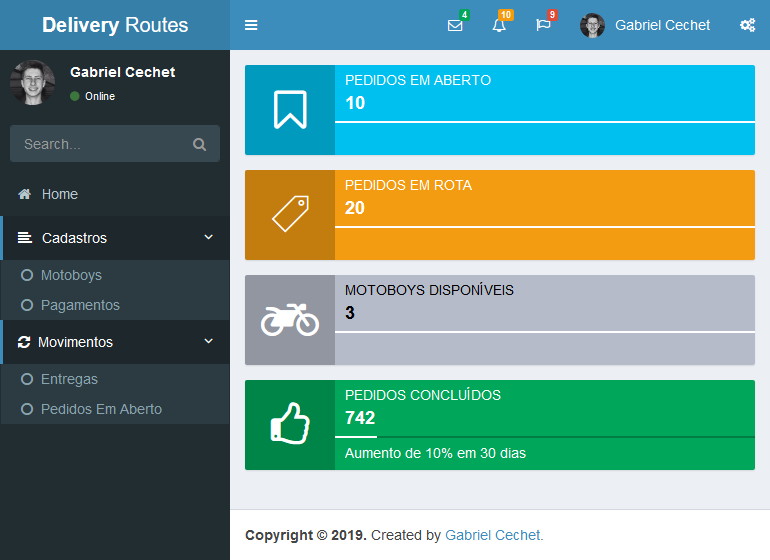
\includegraphics[width=1.0\textwidth]{./dados/figuras/fig13}
    \fonte{Autor}
    \label{fig:drDashboard}
\end{figure}

\newpage
Para desenvolver a \textit{dashboard}
%%% Rev-Madalozzo: listar todos os pacotes de terceiros AdminLTE e PDF


\section{Coleta de dados}
\begin{figure}[H]
    \centering
    \caption{Delivery Routes - Coleta de dados}
    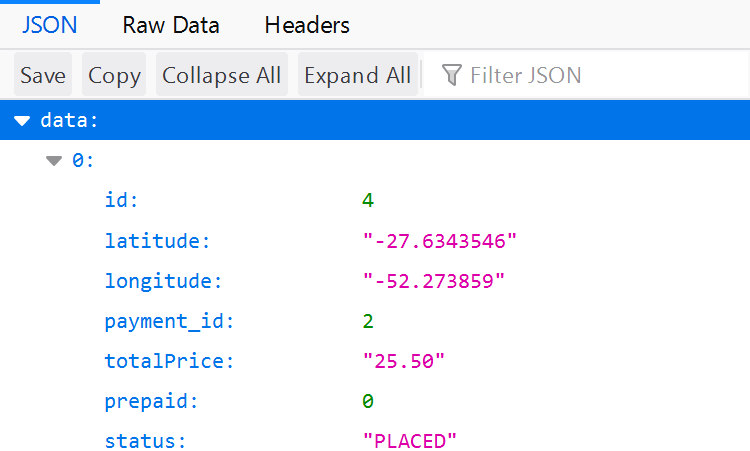
\includegraphics[width=0.6\textwidth]{./dados/figuras/fig14}
    \fonte{Autor}
    \label{fig:drPlacedAPI}
\end{figure}


\newpage
\section{Consulta de dados}
No momento em que a tela retratada na \autoref{fig:drAPIorder} inicia, um serviço de consulta para capturar informações do pedido requerido é executado. Esse serviço realiza uma requisição \textit{GET} na rota \textit{/order/\{id\}}, parametrizada para receber o código do pedido no estabelecimento, integrado pelo sistema anteriormente.

Nesse momento os possíveis status do pedido poderem ser: 
\\ \textit{INTEGRATED}, \textit{CANCELLED}, \textit{DISPATCHED}, \textit{DELIVERED} ou \textit{CONCLUDED}.

\begin{figure}[H]
    \centering
    \caption{Delivery Routes - API - order}
    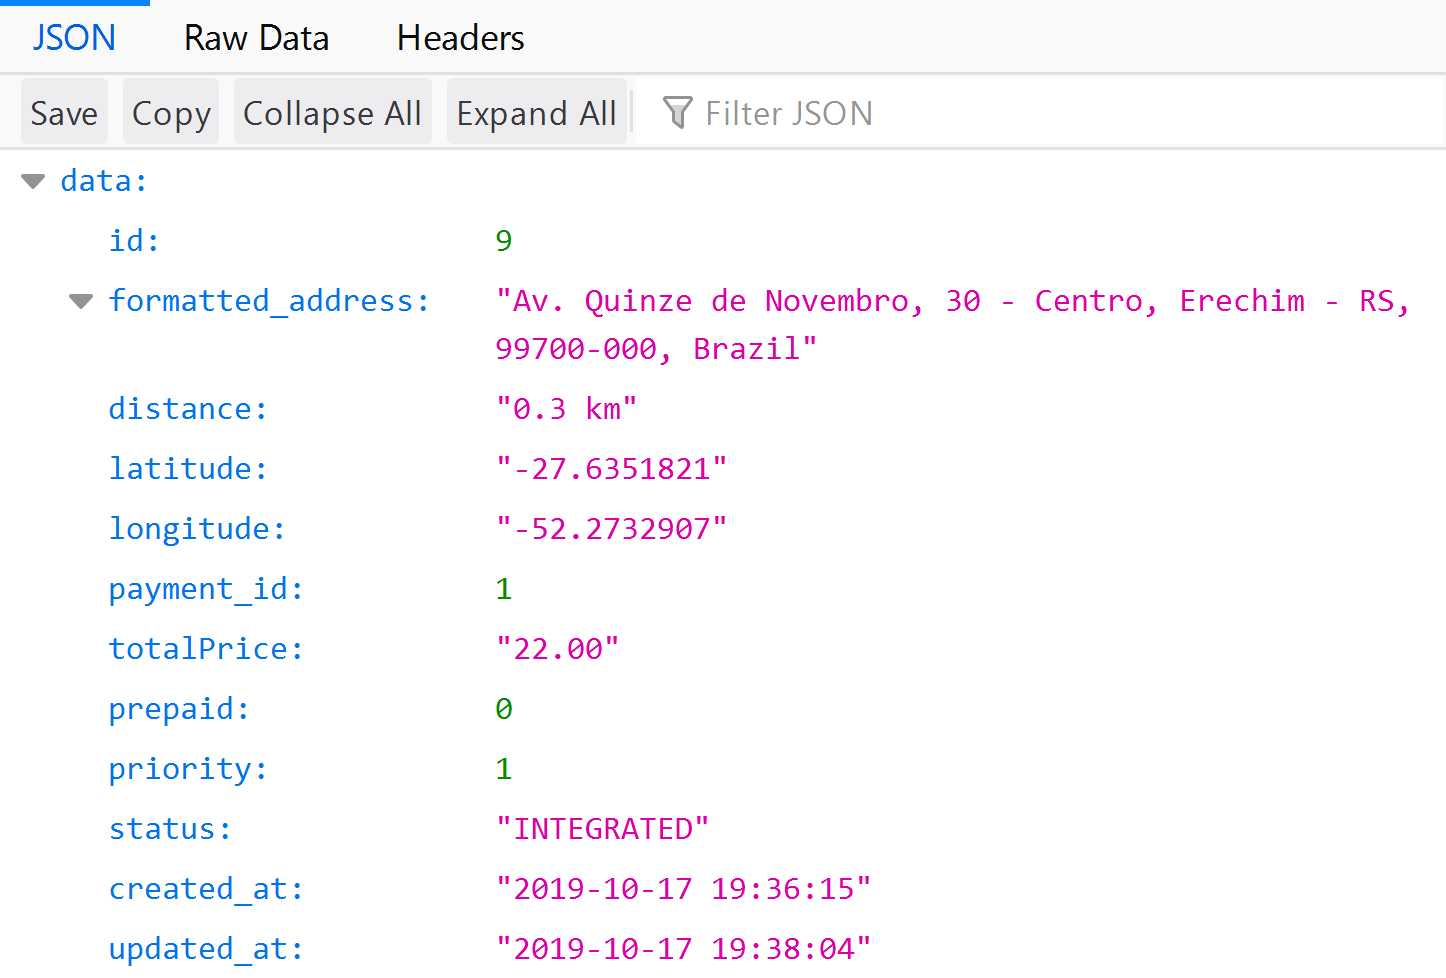
\includegraphics[width=0.9\textwidth]{./dados/figuras/fig22}
    \fonte{Autor}
    \label{fig:drAPIorder}
\end{figure}

Como resultado dessa consulta (como demonstra o \autoref{alg:getOrder}), o servidor retorna o objeto requisitado (em formato JSON) com os respectivos dados solicitados pela rota, por meio da ferramenta \textit{Resources}, exercendo a sua função como um camada de tratamento entre o Eloquent ORM e as respostas JSON que são expostas pela API. Essas classes, criadas ao executar o comando \textit{php artisan make:resource OrdersResource} através do Artisan, permitem transformar facilmente, \textit{models} e \textit{collections} em JSON.

\begin{lstlisting}[caption={Delivery Routes - Route order}, style=htmlcssjs, label=alg:getOrder]
Route::get('/order/{id}', function ($order_id) {
    return new OrdersResource(Order::find($order_id));
});
\end{lstlisting}

\newpage
\section{Módulo de entrega}
Neste módulo é apresentada a usabilidade do sistema por parte do motoboy, realizando a visualização da rota de entrega denominada para o momento.

\subsection{Tracking de entregas}
O primeiro status de uma entrega obrigatoriamente será \textit{CONFIRMED}, isso indica que a mesma foi planejada, visualizada e gerada pelo módulo de gerenciamento. Posteriormente a isso, a comanda (\autoref{fig:drCupom}) é impressa e então o fluxo de \textit{tracking} do pedido é iniciado (\autoref{fig:drFluxoPedido}).

 \begin{figure}[H]
    \centering
    \caption{Delivery Routes - Comanda do pedido}
    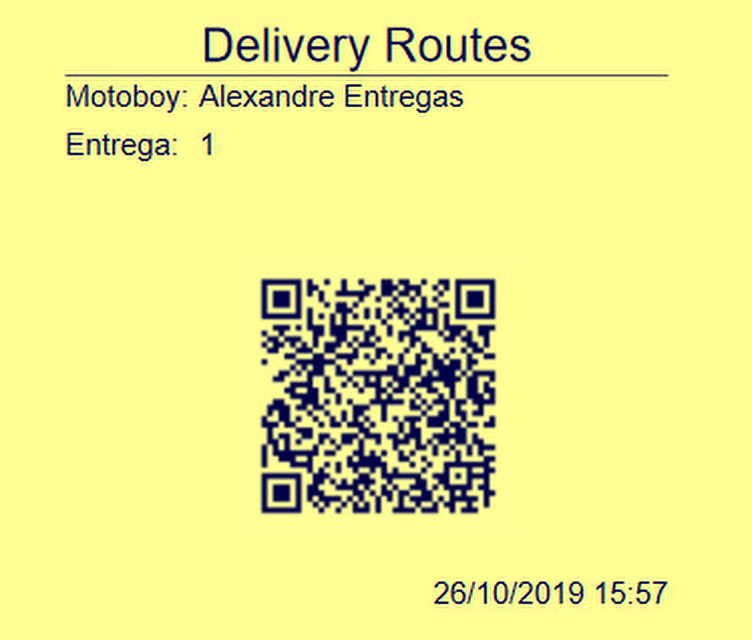
\includegraphics[width=0.4\textwidth]{./dados/figuras/fig24}
    \fonte{Autor}
    \label{fig:drCupom}
\end{figure}

\begin{figure}[H]
    \centering
    \caption{Delivery Routes - Fluxo do pedido}
    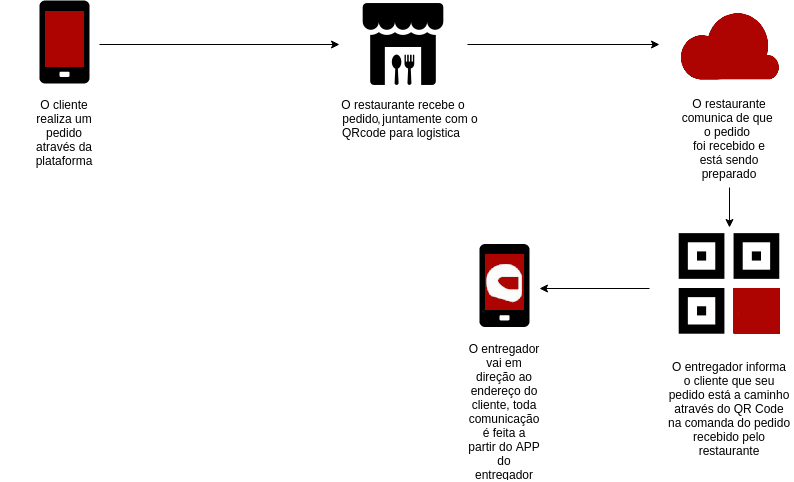
\includegraphics[width=0.85\textwidth]{./dados/figuras/fig25}
    \fonte{Adaptada de \citeonline{iFood}}
    \label{fig:drFluxoPedido}
\end{figure}

Neste cenário, ao ler o código QR impresso na comanda o motoboy é direcionado para a rota: \textit{/deliveries/{id}/dispatched} (\autoref{alg:funcDispatched}), alterando seu status para \textit{DISPATCHED} e executando uma nova rota: \textit{/deliveries/{id}/view}, onde o parâmetro solicitado para ambas é o código da entrega.

\begin{lstlisting}[caption={Delivery Routes - Função de despacho da entrega}, style=htmlcssjs, label=alg:funcDispatched]
public function dispatched($id) {
    $delivery = Delivery::find($id);
    $delivery->update(['status' => 'DISPATCHED']);
    return view('deliveries.view', compact('delivery'));
}
\end{lstlisting}

Logo após o despacho da entrega, é apresentada na tela no \textit{smartphone} do motoboy a representação, distância e tempo de deslocamento do percurso que deve ser percorrido na entrega desejada (\autoref{fig:drRotaEntregaInicio} e \autoref{fig:drRotaEntrega}).

\begin{figure}[H]
    \centering
    \caption{Delivery Routes - Despacho da entrega}
    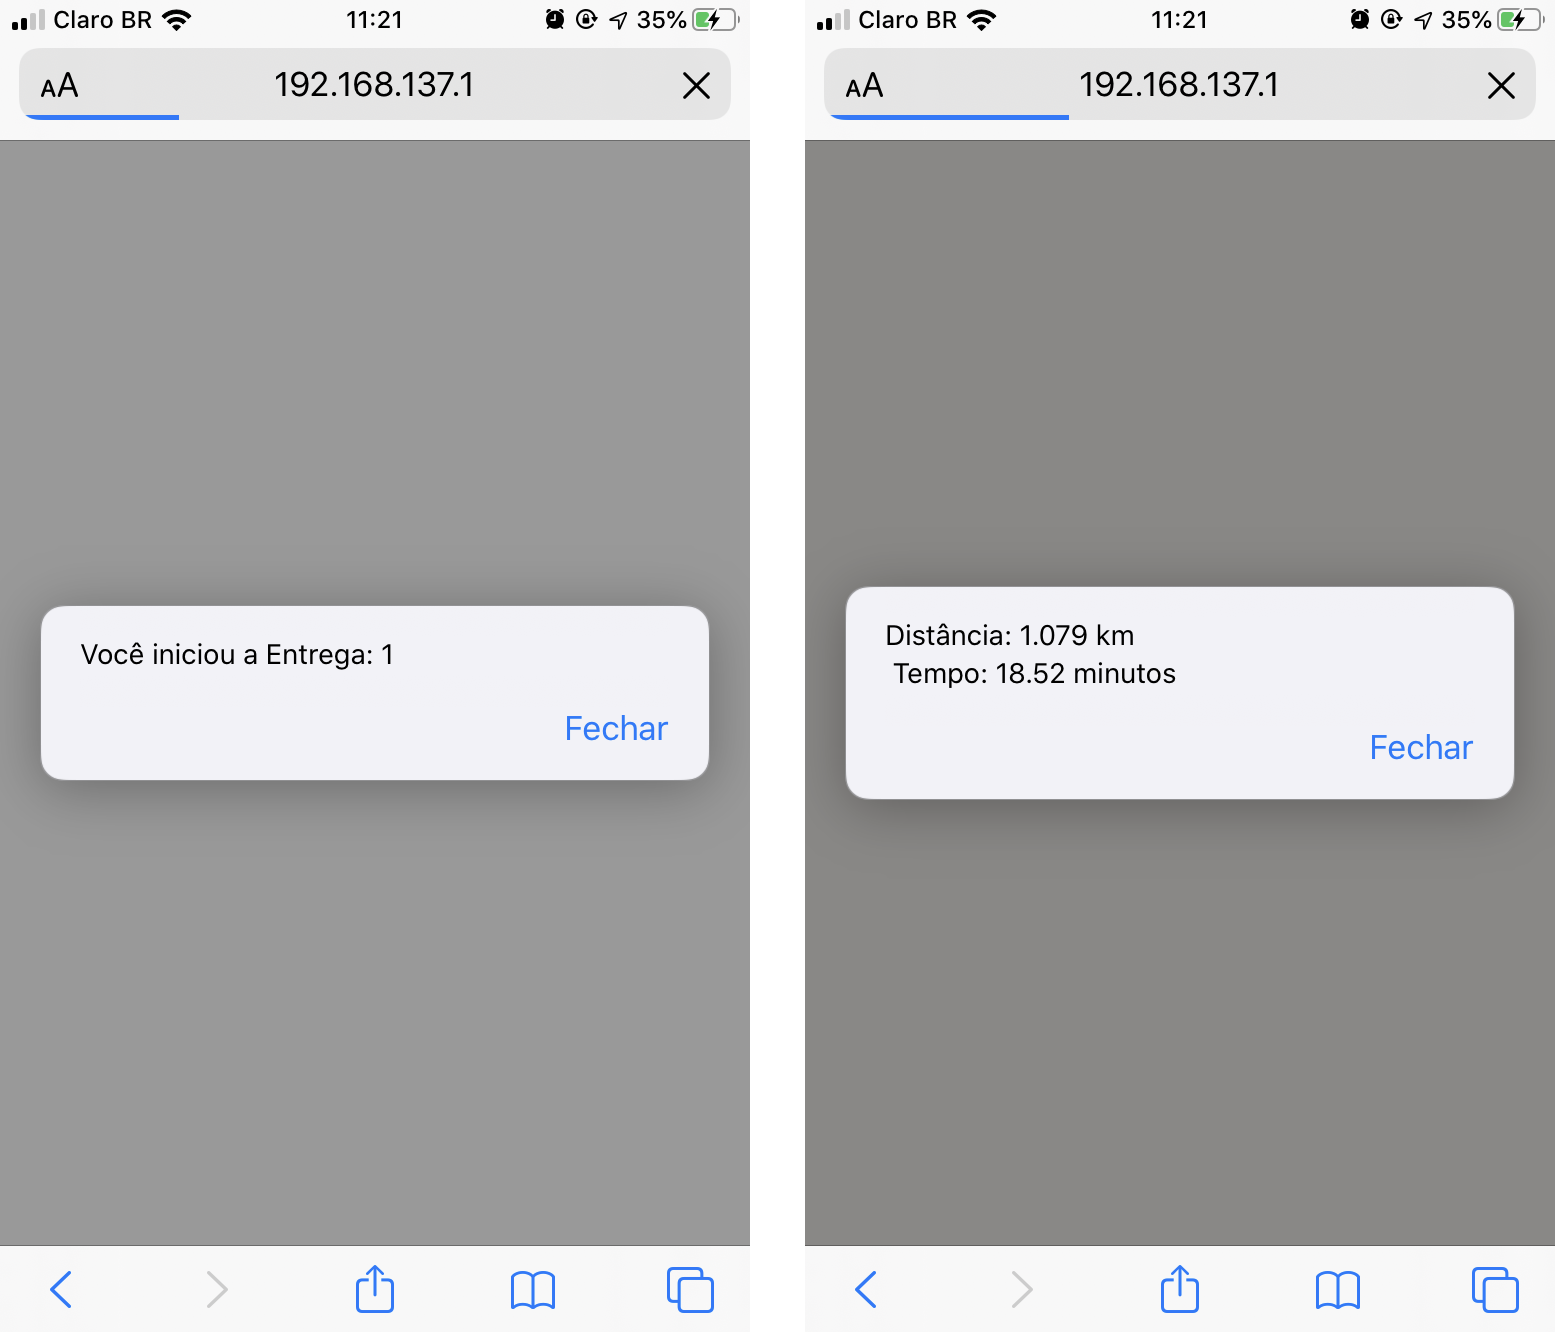
\includegraphics[width=0.9\textwidth]{./dados/figuras/fig28}
    \fonte{Autor}
    \label{fig:drRotaEntregaInicio}
\end{figure}

\newpage
\begin{figure}[H]
    \centering
    \caption{Delivery Routes - Mapa da entrega}
    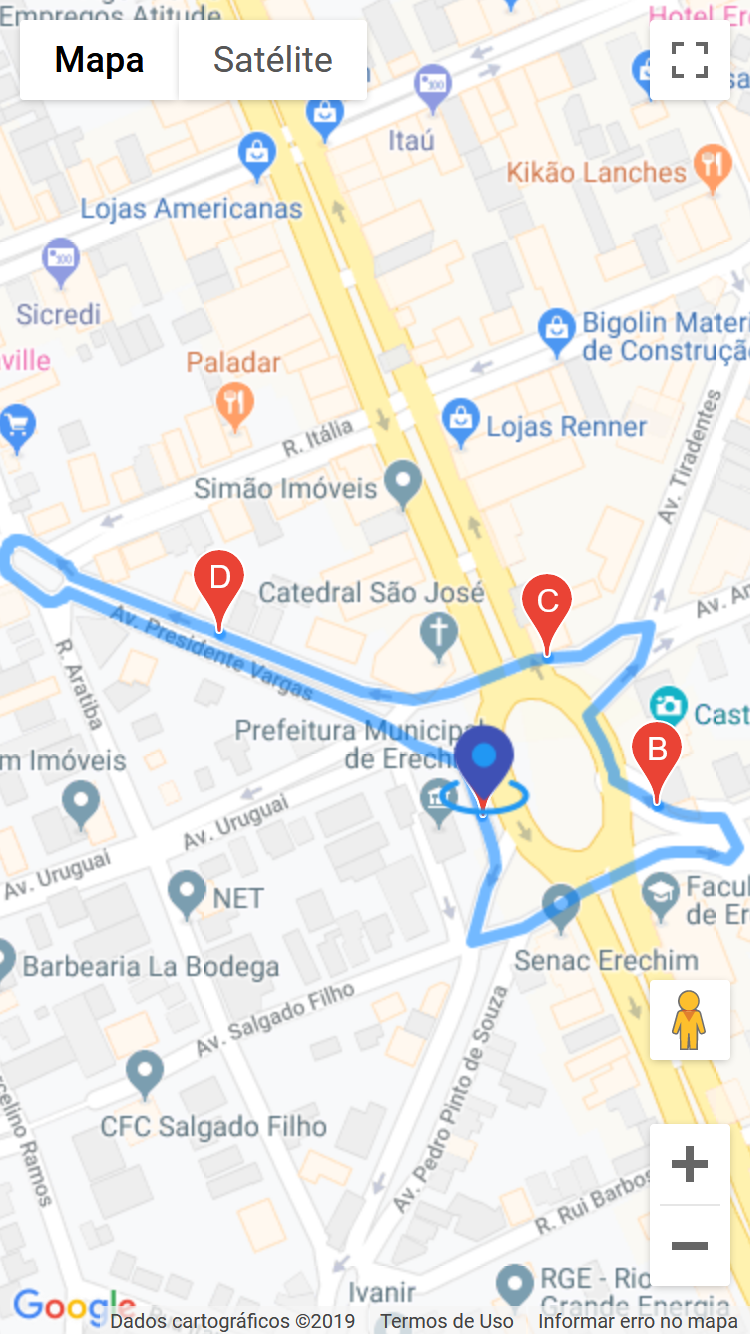
\includegraphics[width=0.8\textwidth]{./dados/figuras/fig27}
    \fonte{Autor}
    \label{fig:drRotaEntrega}
\end{figure}

\newpage
Para obter a rota entre dois pontos e exibi-la no mapa, é necessário utilizar o serviço da \textit{Google Directions} API. Lendo a sua documentação, verificou-se necessário a implementação das classes \textit{google.maps.DirectionsService} e o \textit{google.maps.DirectionsRenderer}.

Começando pelo \textit{DirectionsService}, o seu funcionamento é bem simples. Basta informar um objeto \textit{google.maps.DirectionsRequest}, o qual irá conter o ponto de origem e destino (\autoref{alg:currentPosition}), e o meio de transporte (carro, a pé, bicicleta ou transporte público), que ele irá retornar um objeto \textit{google.maps.DirectionsResult}, o qual contém as informações da rota, e o \textit{google.maps.DirectionsStatus}, que por sua vez define o estado final da requisição. Ele pode indicar sucesso (\textit{OK}), sem resultados (\textit{ZERO\_RESULTS}), erro (\textit{INVALID\_REQUEST} ou \textit{REQUEST\_DENIED}), etc.

\begin{lstlisting}[caption={Delivery Routes - Função de localização do usuário}, style=htmlcssjs, label=alg:currentPosition]
navigator.geolocation.getCurrentPosition(position);
function success(position) {
    currentPosition = new google.maps.LatLng(position.coords.latitude, position.coords.longitude);
};
\end{lstlisting}

Para adicionar os pontos de parada durante a rota, adquiridos através da rota: \textit{/delivering/{id}} (\autoref{alg:pedidosEntrega}), que retorna todos os pedidos da entrega solicitada, é preciso informar uma lista de objetos \textit{google.maps.DirectionsWaypoint} (\autoref{alg:waypoints}), que são alguns pontos pré-definidos no meio do trajeto no objeto \textit{DirectionsRequest} antes de passá-lo para o \textit{directionsService.route}.

\begin{lstlisting}[caption={Delivery Routes - Route pedidos da entrega}, style=htmlcssjs, label=alg:pedidosEntrega]
Route::get('/delivering/{id}', function ($delivery_id) {
    return new OrdersResource(DB::table('orders')
    ->leftJoin('deliveries_orders', 'orders.id', '=', 
    'deliveries_orders.order_id')
    ->where('deliveries_orders.delivery_id', $delivery_id)->get());
});
\end{lstlisting}

\begin{lstlisting}[caption={Delivery Routes - Preenchimento dos pontos de parada}, style=htmlcssjs, label=alg:waypoints]
$.getJSON(json, function(pontos) {
    $.each(pontos.data, function(index, ponto) {
        waypoints[position] = {
            'location': new google.maps.LatLng(ponto.latitude, ponto.longitude)
        };
    });
});
\end{lstlisting}

\newpage
Já o \textit{DirectionsRenderer}, basicamente, fica responsável por renderizar o resultado fornecido pelo \textit{DirectionsService} (\autoref{alg:directionsService}).

\begin{lstlisting}[caption={Delivery Routes - Requisição de renderização do mapa}, style=htmlcssjs, label=alg:directionsService]
var request = {
    origin: currentPosition,
    waypoints: waypoints,
    destination: currentPosition,
    travelMode: google.maps.TravelMode.DRIVING
};

directionsService.route(request, function(result, status) {
    if (status == google.maps.DirectionsStatus.OK) {
        directionsDisplay.setDirections(result);
    }
});
\end{lstlisting}

O cálculo de distância e tempo (\autoref{alg:computeTotalDistance}), exibido na \autoref{fig:drRotaEntregaInicio}, é a última etapa. Nele é computado o tempo de deslocamento entre os pontos e também o tempo dos trâmites de entrega do produto para o cliente final, estimado em 5 minutos cada.

\begin{lstlisting}[caption={Delivery Routes - Função de cálculo do deslocamento}, style=htmlcssjs, label=alg:computeTotalDistance]
function computeTotalDistance(result) {
    var totalDist = 0;
    var totalTime = -300; // retorno
    var myroute = result.routes[0];
    for (i = 0; i < myroute.legs.length; i++) {
        totalDist += myroute.legs[i].distance.value;
        totalTime += myroute.legs[i].duration.value;
        totalTime += 300;
    }
}
\end{lstlisting}

A maioria dos produtos da Google são pagos, porém há um crédito (200 dólares para uso mensal gratuito, que condizem com até 28 mil carregamentos no valor de 7 dólares por milhar) disponível no momento da requisição dos serviços, que vai sendo debitado na medida que é requisitado. Não é cobrado valor algum até que esse crédito seja totalmente utilizado. Ele pode ser usado no \textit{Maps}, no \textit{Routes} ou no \textit{Places}. Para fins de uso e cobrança, é necessário uma chave da API JavaScript do \textit{Google Maps}. A chave da API é um identificador exclusivo usado para autenticar solicitações associadas ao projeto.

\newpage
\section{Controller}
Esse domínio do MVC é responsável por direcionar os \textit{requests} conforme a regra de negócio, também de acordo com a arquitetura do projeto, ele é responsável por autenticar o usuário e garantir que as rotas do sistema estão sendo acessadas por alguém autenticado. 

No caso dos controladores, também foi criado um específico para cada classe, onde ele será responsável por direcionar os pedidos conforme a especificidade. Dessa forma, podemos utilizar como exemplo o caso da classe \textit{Motoboy}, com o controlador representado no \autoref{alg:controllerMotoboy}.

\begin{lstlisting}[caption={Delivery Routes - Exemplo de um Controller: Motoboy}, style=htmlcssjs, label=alg:controllerMotoboy]
<?php
class MotoboysController extends Controller {
    public function index() {
        $item = Motoboy::all();
        return view('motoboys.index', ['motoboys' => $item]);
    }
    public function create() {
        return view('motoboys.create');
    }
    public function store(MotoboysRequest $request) {
        Motoboy::create($request->all());
        Request()->session()->flash('mensagem-sucesso', 'Registro salvo com sucesso.');
        return redirect()->route('motoboys');
    }
    public function destroy($id) {
        Motoboy::find($id)->delete();
        Request()->session()->flash('mensagem-sucesso', 'Registro excluso com sucesso.');
        return redirect()->route('motoboys');
    }
    public function edit($id) {
        $item = Motoboy::find($id);
        return view('motoboys.edit', compact('item'));
    }
    public function update(MotoboysRequest $request, $id) {
        Motoboy::find($id)->update($request->all());
        Request()->session()->flash('mensagem-sucesso', 'Registro salvo com sucesso.');
        return redirect()->route('motoboys');
    }
}
\end{lstlisting}

\newpage
\begin{table}[H]
    \centering
    \caption{Delivery Routes - Exemplo de router do back-end
    \label{tab:drRoutes}}
\begin{tabular}{llp{9.2cm}l}
\toprule
\textbf{Método} & \textbf{URI} & \textbf{Ação} \\
\midrule
GET & / & Exibe a dashboard do aplicativo. \\
GET & register & Exibe o formulário de inscrição do aplicativo. \\
POST & register & Manipula uma solicitação de registro para o aplicativo. \\
GET & login & Exibe o formulário de login do aplicativo. \\
POST & login & Manipula uma solicitação de login para o aplicativo. \\
POST & password/email & Envia um link de redefinição para o usuário especificado. \\
GET & password/reset & Exibe o formulário para solicitar um link de redefinição de senha. \\
GET & password/reset/\{token\} & Exibe a visualização de redefinição de senha para o token fornecido. \\
POST & password/reset & Redefine a senha do usuário fornecido. \\
POST & logout & Desconecta o usuário do aplicativo. \\
GET & motoboys & Exibe a listagem de motoboys cadastrados. \\
GET & motoboys/create & Exibe o formulário para cadastrar um novo motoboy. \\
POST & motoboys/store & Manipula uma solicitação de cadastro de um motoboy. \\
GET & motoboys/\{id\}/edit & Manipula uma solicitação de edição de um motoboy. \\
PUT & motoboys/\{id\}/update & Manipula uma solicitação de atualização de um motoboy. \\
GET & motoboys/\{id\}/destroy & Manipula uma solicitação de exclusão de um motoboy. \\
GET & payments & Exibe a listagem de pagamentos cadastrados. \\
GET & payments/create & Exibe o formulário para cadastrar um novo pagamento. \\
POST & payments/store & Manipula uma solicitação de cadastro de um pagamento. \\
GET & payments/\{id\}/edit & Manipula uma solicitação de edição de um pagamento. \\
PUT & payments/\{id\}/update & Manipula uma solicitação de atualização de um pagamento. \\
GET & payments/\{id\}/destroy & Manipula uma solicitação de exclusão de um pagamento. \\
GET & orders & Exibe a listagem de pedidos disponíveis para integração. \\
GET & order/\{id\} & Retorna os atributos do pedido desejado em formato JSON. \\
GET & deliveries & Exibe a listagem de entregas cadastradas. \\
GET & deliveries/store & Manipula uma solicitação de cadastro de uma entrega. \\
GET & deliveries/\{id\}/ticket & Manipula uma solicitação de impressão do ticket de uma entrega. \\
GET & delivering/\{id\} & Retorna os atributos dos pedidos da entrega desejada em formato JSON. \\
GET & deliveries/\{id\}/view & Manipula uma solicitação de início de um entrega. \\
GET & deliveries/\{id\}/dispatched & Manipula uma solicitação de despacho de uma entrega. \\
GET & deliveries/\{id\}/concluded & Manipula uma solicitação de conclusão de uma entrega. \\
GET & deliveries/\{id\}/cancelled & Manipula uma solicitação de cancelamento de uma entrega. \\
\bottomrule
\end{tabular}
    \fonte{Autor}
\end{table}

\newpage
Além de implementar os controladores de todas as classes, foi necessário estabelecer quais seriam as rotas e quais controles serão chamados de acordo com a rota. Para isso o \textit{framework} Laravel disponibiliza um \textit{router}, responsável por organizar as rotas e direcioná-las de acordo com o controlador (\autoref{tab:drRoutes}). Nesse mesmo \textit{router}, também direciona as rotas de autenticação caso o usuário não esteja logado.

\section{Integração da ferramenta}
As APIs simplificam a forma como os desenvolvedores integram novos componentes de aplicações a uma arquitetura preexistente. Por isso, elas ajudam na colaboração entre as empresas e as equipes de desenvolvimento. Muitas vezes, as necessidades empresariais mudam rapidamente para responder aos mercados digitais em transformação. Nesse ambiente, a ferramenta desenvolvida pode ser integrada em qualquer nicho de mercado que possua a opção de entrega de seus produtos sob gerenciamento de um sistema já existente e aberto à novas integrações.
%Ajudando a facilitar o dia a dia de estabelecimentos parceiros, que por muitas vezes, tem um fluxo muito grande de pedidos e é necessário uma automação, para uma melhor operação interna e evitar possíveis erros humanos.

Em contato com a equipe de desenvolvimento da plataforma \textit{Kitchen} (iFood), para um momento curto, eles não demonstraram interesse em tentar realizar a integração com o Delivery Routes.

%O trecho de código fonte que é apresentado a seguir demonstra como é o serviço de                login do aplicativo: 
%, conforme apresenta a figura 19 
%, conforme a figura 20 mostra
